Die bisherigen Nächte waren unter Beachtung der Räumlichkeit ganz okay, was nicht heißen soll, man hätte ohne Ohropax auch nur den Hauch einer Chance gehabt zu schlafen.
In dieser war es allerdings ein klein wenig anders.
Gegen 3~Uhr nachts bin ich aufgewacht, weil mir kalt war.
Dabei habe ich ein lautes Brummen vernommen, ähnlich eines Bienenschwarms etwa 5~cm vom Ohr entfernt.
Der Bienenschwarm entpuppte sich als Ventilator, der einen wahnsinnigen Krach machte.
Aber ohne wären wir alle zerlaufen.
Mit dem Kopfkissen im Rücken als Windschutz ging es dann einigermaßen und um 6~Uhr war die Nacht sowieso vorbei.

Relativ pünktlich waren wir im Disneyland Park und dort ging es zügig von Fahrgeschäft zu Fahrgeschäft.
Die Ausgänge der Attraktionen führen immer durch Shops in denen die zugehörige Merchandisingartikel verhökert werden.
Am Splash-Mountain standen zwei kleine gut genährte Prinzessinnen mit uns an, die mehr Ähnlichkeit mit Miss Piggey als mit Anasthasia hatten. 
Als Kind war ich hier schon einmal und hatte deshalb erwartet, wir würden für den Park den gesamten Tag brauchen.
Mit dem interessanten Zeug waren wir dann aber schon auf 3~Uhr durch.
\FOREIGN{``My little World''} fehlte noch, aber dafür wollte sich der Christian nicht anstellen.
Also ging es raus und wir buchten den Adventure Park mit dazu.
So wurden aus stolzen 95~\$ noch stolzere 155~\$ \textbf{pro} Nase.
Der Advenure Park ist ähnlich aufgebaut.
Dort haben wir dann auch mal kapiert was es mit diesem \FOREIGN{Fast Pass} auf sich hat.
Anfangs dachten wir man kann sich dafür einkaufen, aber das ist nicht der Fall.
Mit seiner Eintrittskarte zieht man an \FOREIGN{Fast Pass}-Ausgabestationen (\FOREIGN{Delivery}) ein Ticket, das einem erlaubt zu einem in der Zukunf liegenden Zeitraum an der Warteschlange zumindest größtenteils vorbei zu gehen.
Da man nur alle 45~Minuten einen neuen \FOREIGN{Fast Pass} ziehen kann, ist es auch nicht möglich diese zu horten.

Am Abend findet im Adventure Park ab 20~Uhr eine sehenswerte Lichtershow \FOREIGN{``World of Color''} statt und im Disneyland Park nahezu zeitgleich eine Parade, die in einem Feuerwerk über dem Schloss endet, wenn es das Wetter zulässt.
Bei uns war es zu windig.

\newpage
\thispagestyle{empty}
\begin{tikzpicture}[remember picture, overlay]
\node[inner sep=0pt] at (current page.center) {%
	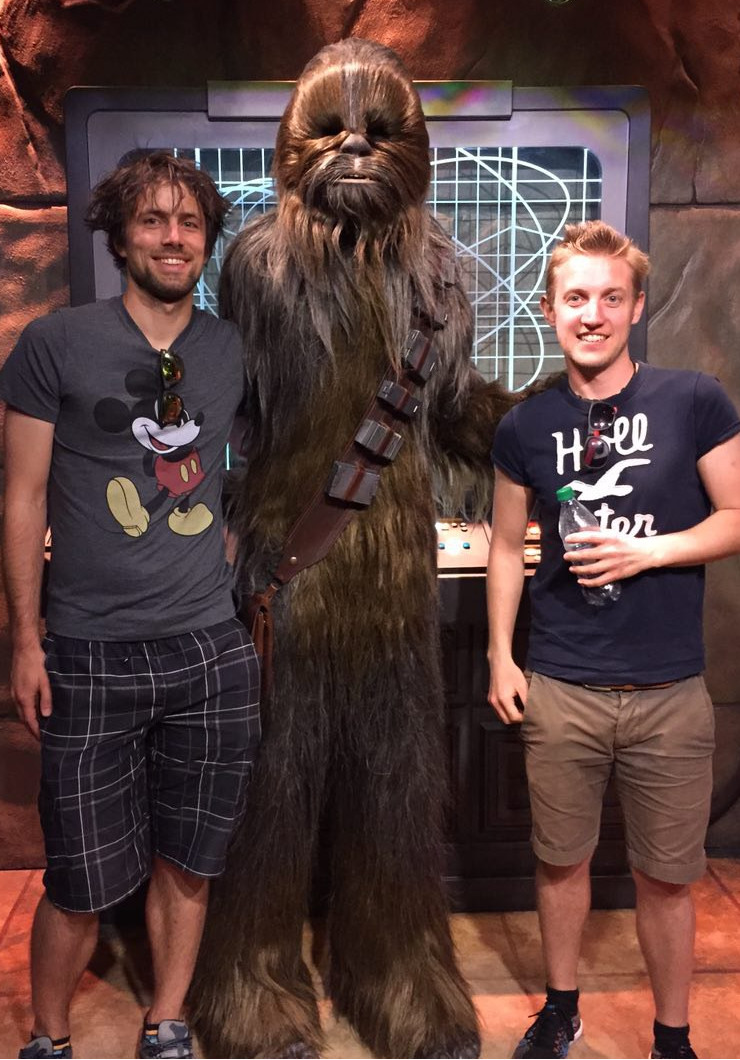
\includegraphics[width=\paperwidth,height=\paperheight]{18/Zottelviech.jpg};%
};
%\node[inner sep=0pt, yshift=.25\paperheight] at (current page.south) {%
%	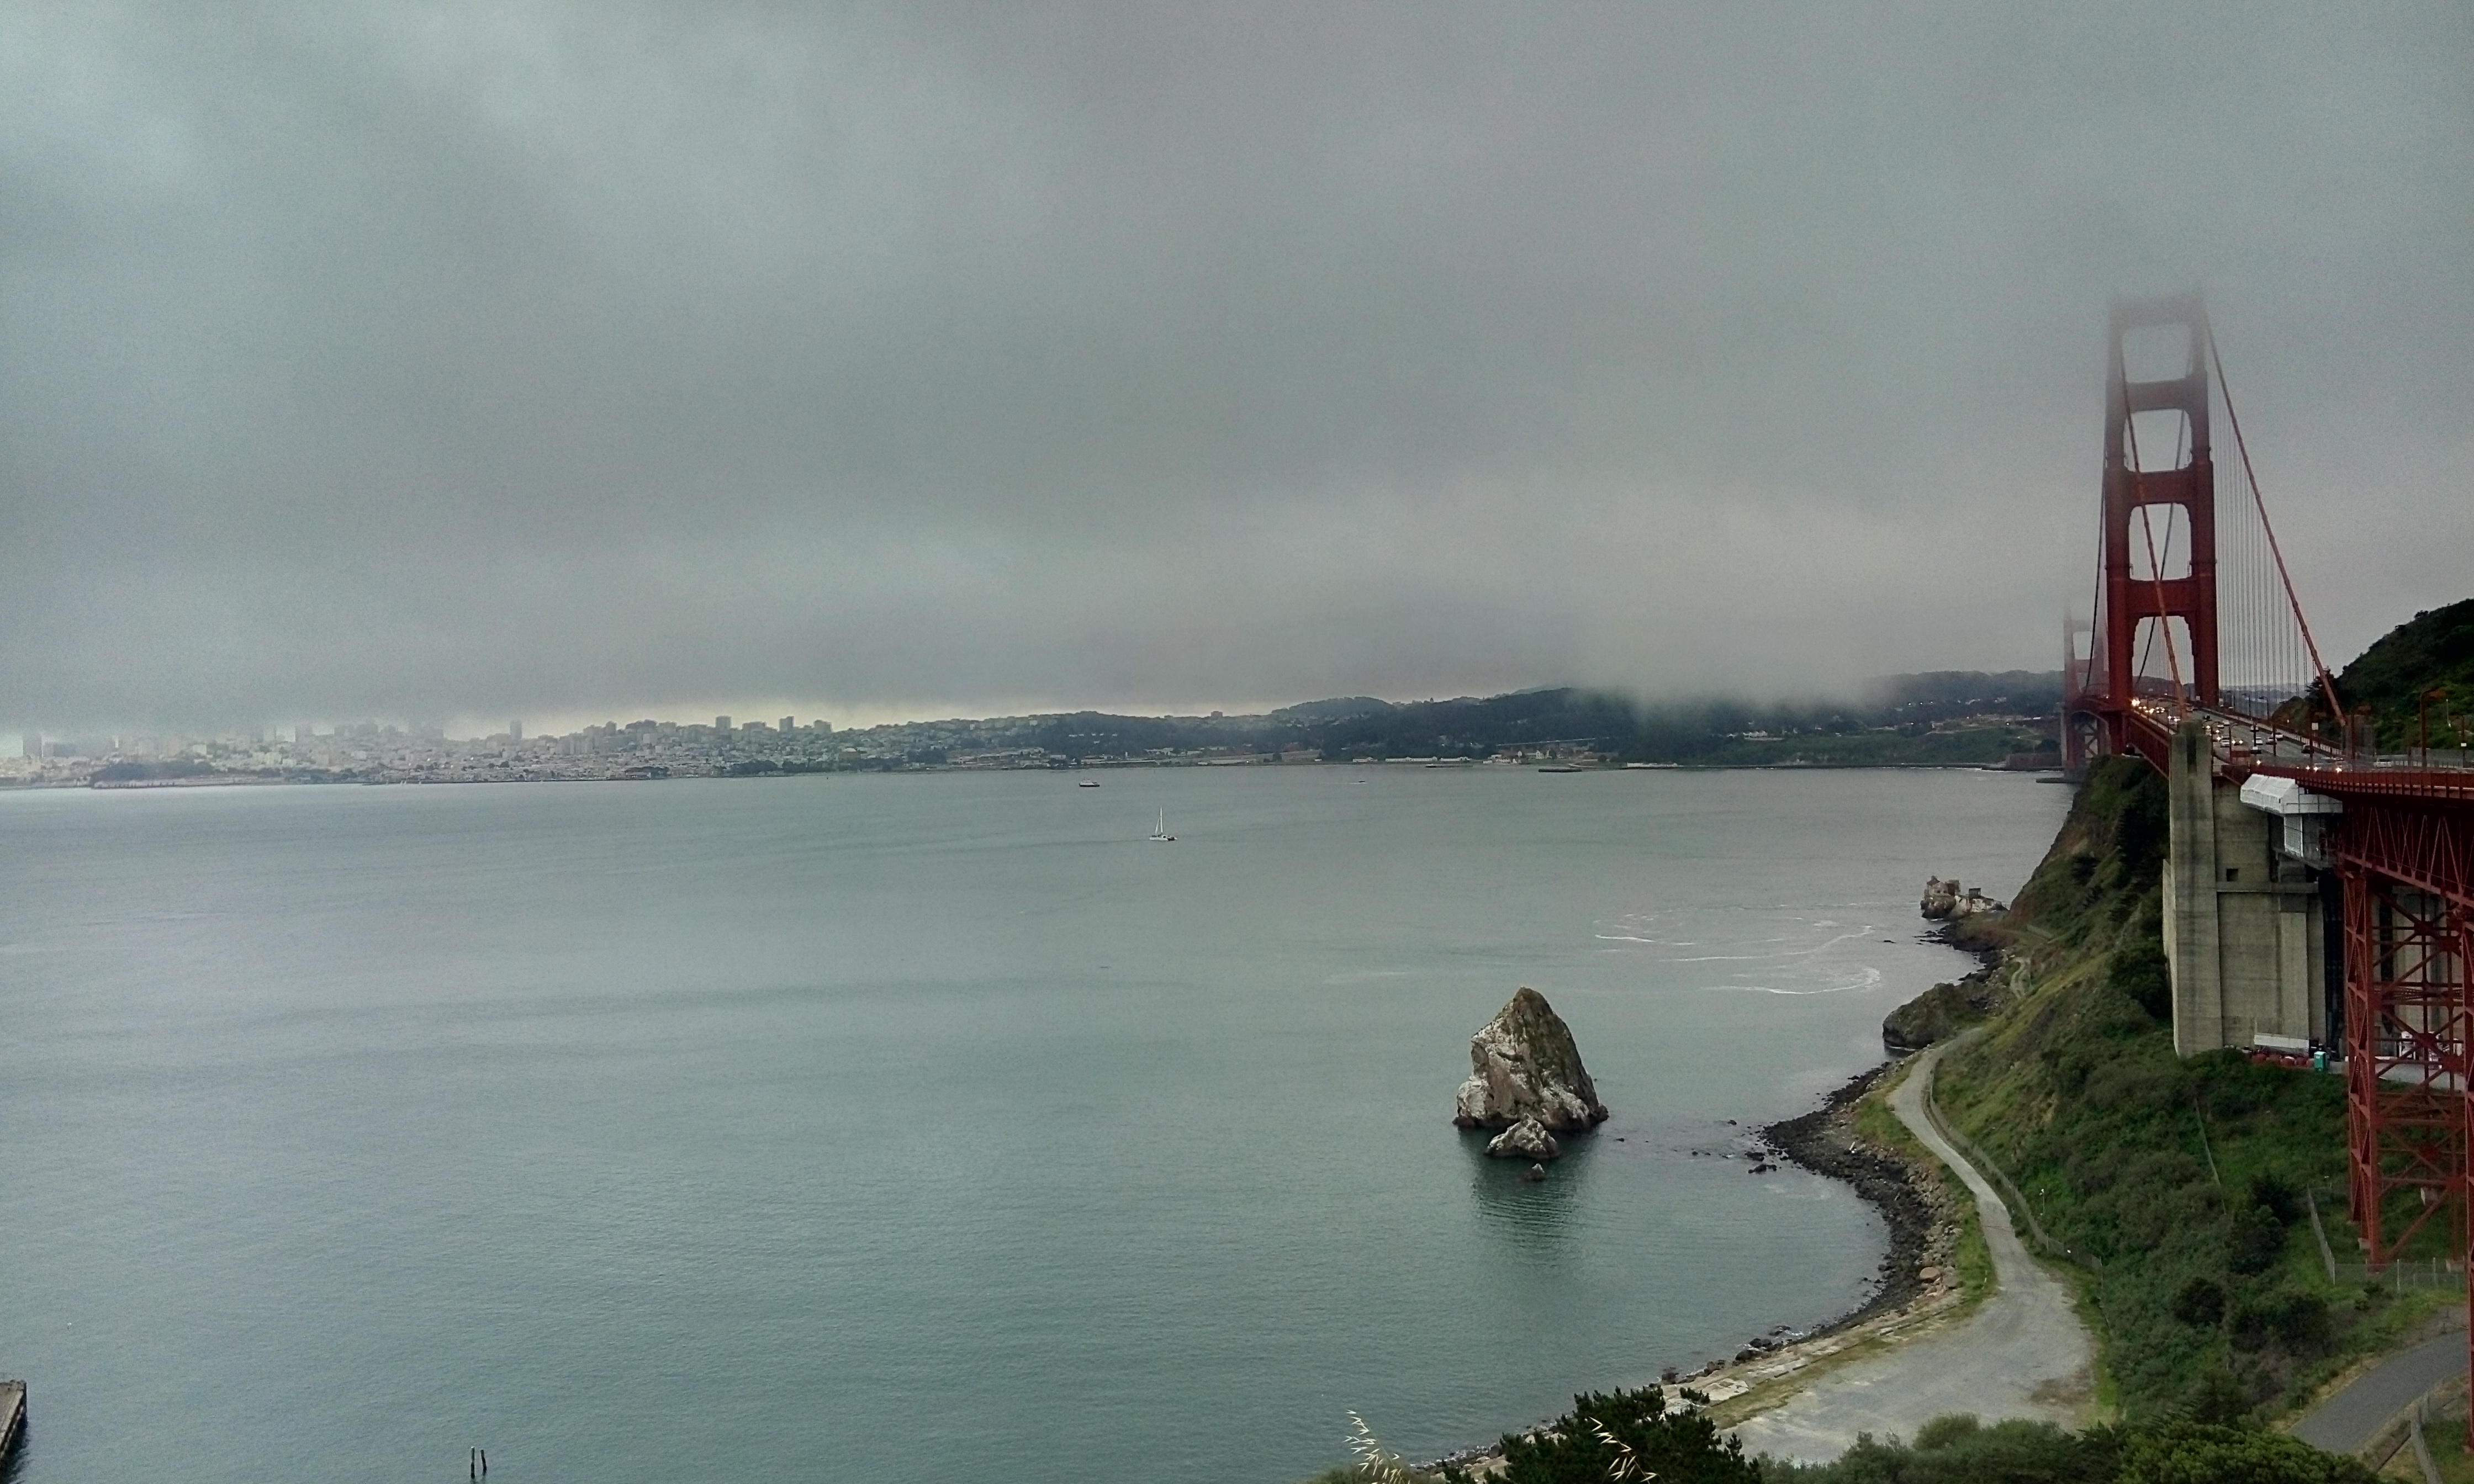
\includegraphics[width=\paperwidth,height=.5\paperheight]{21/image20160420_193101911.jpg};%
%};
\end{tikzpicture}
\newpage


